\documentclass[../thesis/thesis.tex]{subfiles}
\begin{document}

\chapter{Evaluation}
\label{chap:evaluation}

We believe it is possible to produce a VC investment screening system that is efficient, robust and powerful. In the previous chapter, we describe the development and structure of such a system. Our system is based around identifying startup companies that are likely to receive additional funding or a liquidity event (exit) in a given forecast window. This system can generate statistics and make recommendations that may assist VC firms to efficiently and effectively screen investment candidates. In our literature review, we determined that our proposed system must satisfy three criteria to be useful to VC firms: efficiency, robustness and predictive power. In this chapter, we evaluate our system against that criteria.

\begin{enumerate}

\item Pipeline Selection. In the previous step, we generated a cross-section of candidate pipelines with different hyperparameters. In this step, we use Area under the \gls{pr} curve to rank these candidate pipelines and test the best pipelines (finalist pipelines) over a number of different dataset slices. This process ensures we select pipelines that are robust with respect to time. We aggregate the results for each finalist pipeline across these dataset slices and rank the finalist pipelines on their overall performance, so we can select the best pipeline for further evaluation. We don't observe significant variance in the pipelines on aggregate against the dataset slices, but there is variance within the individual pipelines. Our results suggest that it is optimal to evaluate the top 3-5 candidate pipelines in this manner.

\item Model Evaluation. In the previous step, we selected the best pipeline with respect to the robustness of its performance over time. In this step, we evaluate the performance of the models produced by the best pipeline. We use the pipeline to fit a model to a dataset sliced from the master database. We apply this model to another feature vector from the master database and make predictions. We score these predictions against truth values derived from the held-out test database (collected April 2017). This process is performed multiple times to evaluate our three primary criteria: efficiency, robustness, and predictive power. The experiments are as follows: efficiency, the pipeline is fitted to datasets of various sample sizes; robustness, the pipeline is fitted to datasets from various time slices; and predictive power, the forecast window between the feature vector and outcome is varied. Results of these experiments are described in detail in Chapter~\ref{chap:evaluation}.

\end{enumerate}

Firstly, we evaluate efficiency by exploring the learning curves of our classification techniques and whether there is sufficient data to produce reliable statistics. We also evaluate efficiency with respect to accuracy at different levels of feature abstraction (e.g. feature grouping based on our conceptual framework). Secondly, we evaluate robustness by evaluating our models against multiple reverse-engineered historical datasets and measuring their variance. Thirdly, we evaluate predictive power by testing different forecast windows outcomes and evaluating our models’ accuracy for startups at different stages of their development lifecycle. Finally, we discuss our findings more broadly and their implications for investors and future research into startup investment and performance.

\section{Pipeline Selection}

In the previous chapter, we developed a system that generated a cross-section of candidate pipelines with different hyperparameters. In this step, we terank these candidate pipelines and evaluate the best pipelines (finalist pipelines) over a number of different dataset slices. This process, depicted in Figure~\ref{fig:evaluation:pipeline_selection}, ensures that our final pipeline is robust in their performance with respect to time. We aggregate the results for each finalist pipeline across these dataset slices and rank the finalist pipelines on their overall performance. Finally, we select the best pipeline.

\begin{figure}[!htb]
    \centering
    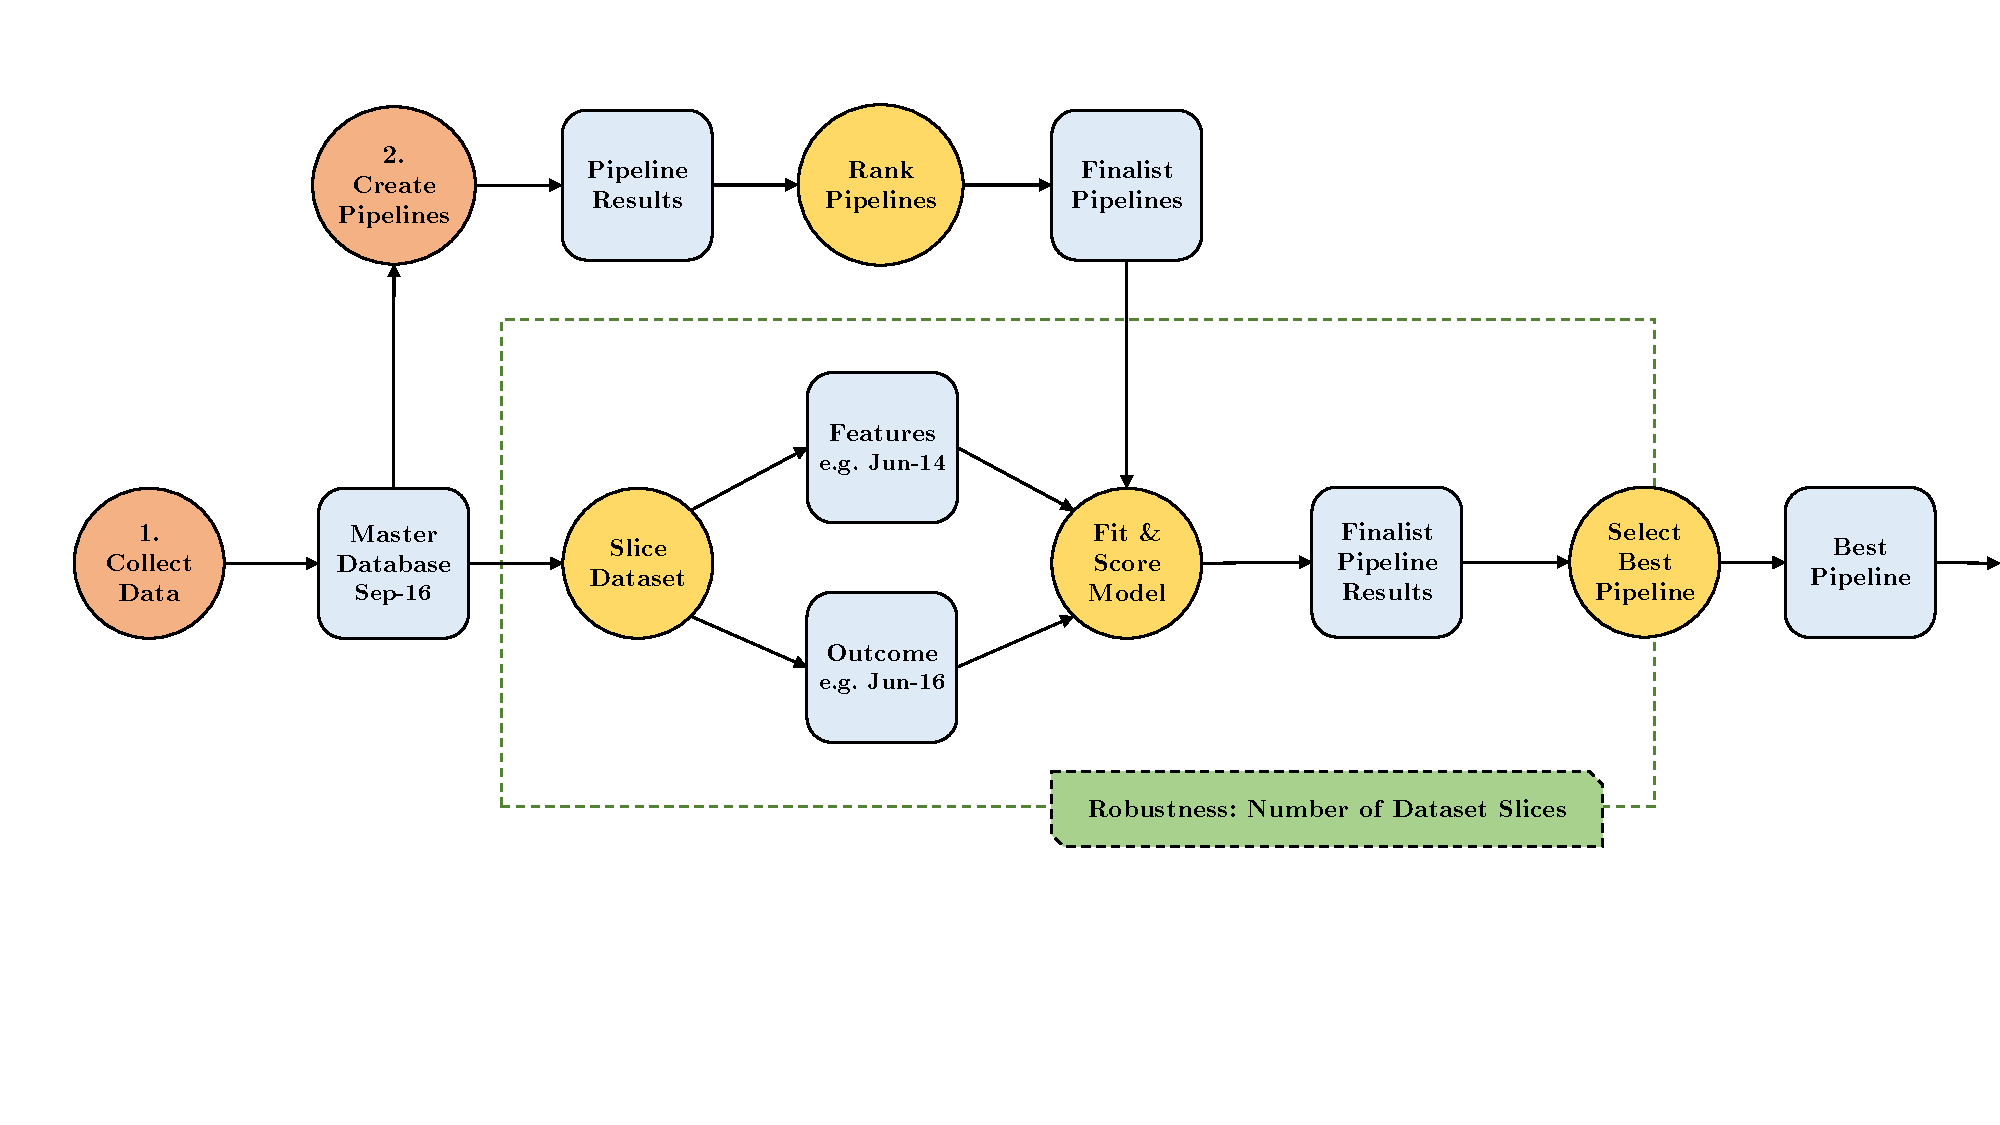
\includegraphics[width=\textwidth]{../figures/evaluation/pipeline_selection}
    \caption[Pipeline selection flowchart]{Pipeline selection overview.}
    \label{fig:evaluation:pipeline_selection}
\end{figure}

First, we need to decide how to narrow our candidate pipelines down to finalist pipelines that we can evaluate further. There are a number of different metrics used to evaluate binary classifiers in machine learning. The most simplistic metric is accuracy but this is rarely used in practice because it gives highly misleading results in the case of imbalanced classes. \Gls{roc} curves are perhaps the mostly commonly used evaluation tool in binary classification, and show how the number of correctly classified positive examples varies with the number of incorrectly classified negative examples. The area under these curves gives a standardised result across a spectrum of decision thresholds. \Gls{pr} curves are similar to \gls{roc} curves but instead map the trade-offs between precision and recall. They are less commonly used than \gls{roc} curves but have been shown to give a more informative picture of an algorithm’s performance under imbalanced classes than \gls{roc} curves \cite{Jesse Davis 2006}. Given our dataset is highly imbalanced (the positive class is approximately 10\%) we decided to proceed with \gls{pr} curves. We will also use this metric to determine which is ultimately the best of our finalist pipelines.

Our hypothesis is that the performance of our classification pipelines may vary with respect to the date that the dataset was collected (in this case, sliced). To study this hypothesis, first we explored variance between the pipelines on aggregate against the slice dates, presented in Figure~\ref{fig:evaluation:selection_agg_slice}. We see little variance on this basis, and we don't observe a relationship between slice date and score.

\begin{figure}[!htb]
    \centering
    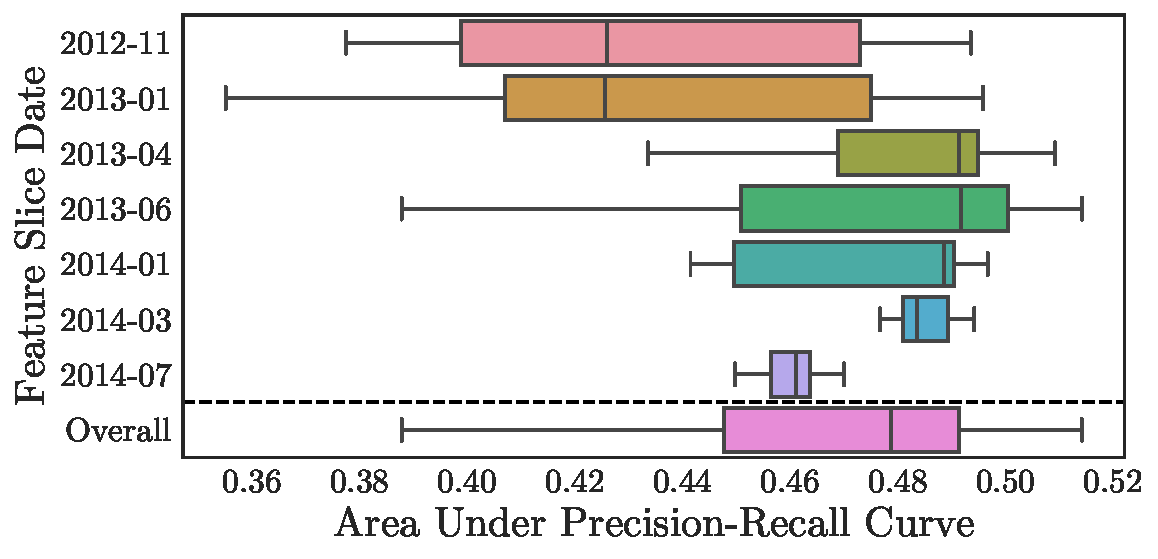
\includegraphics[width=\textwidth]{../figures/evaluation/selection_agg_slice}
    \caption[Pipeline performance by slice date]{}
    \label{fig:evaluation:selection_agg_slice}
\end{figure}

Next, we study the variance within the individual pipelines, presented in Figure~\ref{fig:evaluation:selection_agg_rank}. Here, we can see there is significantly more variance in the scores. Although there is still a strong positive correlation between the pipelines initial ranking and their scores, we can see that there are some individual deviations. Importantly, the top-ranked pipeline from the first stage actually has a lower median score than the second-ranked pipeline. These results suggest that the top 3-5 pipelines should be evaluated in this manner to ensure that the best pipeline is selected.

\begin{figure}[!htb]
    \centering
    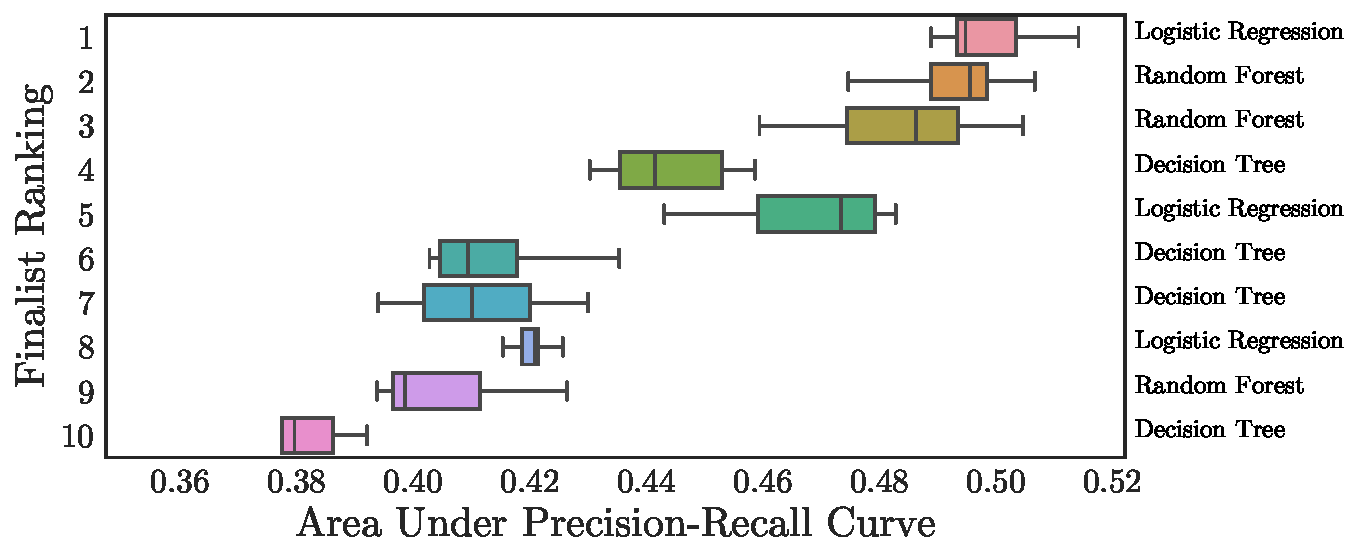
\includegraphics[width=\textwidth]{../figures/evaluation/selection_agg_rank}
    \caption[Overview of finalist pipeline performance]{}
    \label{fig:evaluation:selection_agg_rank}
\end{figure}

The best candidate pipeline is depicted in Table~\ref{fig:evaluation:best_hyperparameters}. We adopted this pipeline configuration for our following experiments.

\begin{table}[!htb]
    \centering
    \scalebox{0.8}{\begin{tabular}{lll} \toprule
Step            & Parameter             & Values                        \\ \midrule
Imputer         & Strategy              & Mode                          \\
Transformer     & Function              & SQRT                          \\
Scaler          & Function              & StandardScaler                \\
Extractor       & Components            & Range (1, 20)                 \\
Random Forest   & Class Weight          & Balanced                      \\
Random Forest   & Criterion             & Entropy                       \\
Random Forest   & Boostrap              & True                          \\
Random Forest   & Estimators            & Range (50, 100)               \\
Random Forest   & Max Depth             & Range (5, 10)                 \\
Random Forest   & Max Features          & SQRT(N_Features)              \\
Random Forest   & Min Samples Split     & 2                             \\
Random Forest   & Min Samples Leaf      & 1                             \\
Random Forest   & Min Weight Leaf       & 0                             \\
Random Forest   & Max Leaf Nodes        & None                          \\
Random Forest   & Min Impurity Split    & 1e-7                          \\
\bottomrule \end{tabular}
}
    \caption[Hyperparameters of best pipeline]{}
    \label{fig:evaluation:best_hyperparameters}
\end{table}

\section{Model Evaluation}

In the previous step, we selected the best pipeline with respect to the robustness of its performance over time. In this step, we evaluate the best pipeline's performance on a held-out test dataset, depicted in \ref{fig:evaluation:pipeline_evaluation}. We use the pipeline to fit a model to a dataset sliced from the master database. We apply this model to another feature vector from the master database and make predictions. We score these predictions against truth values derived from the held-out test database (c. Apr-17). This process is performed multiple times to evaluate our three primary criteria: efficiency, robustness, and predictive power. The experiments are as follows: efficiency, the pipeline is fitted to datasets of various sample sizes; robustness, the pipeline is fitted to datasets from various time slices; and predictive power, the forecast window between the feature vector and outcome is varied. Results of these experiments are described in detail in Chapter~\ref{chap:evaluation}.

\begin{figure}[!htb]
    \centering
    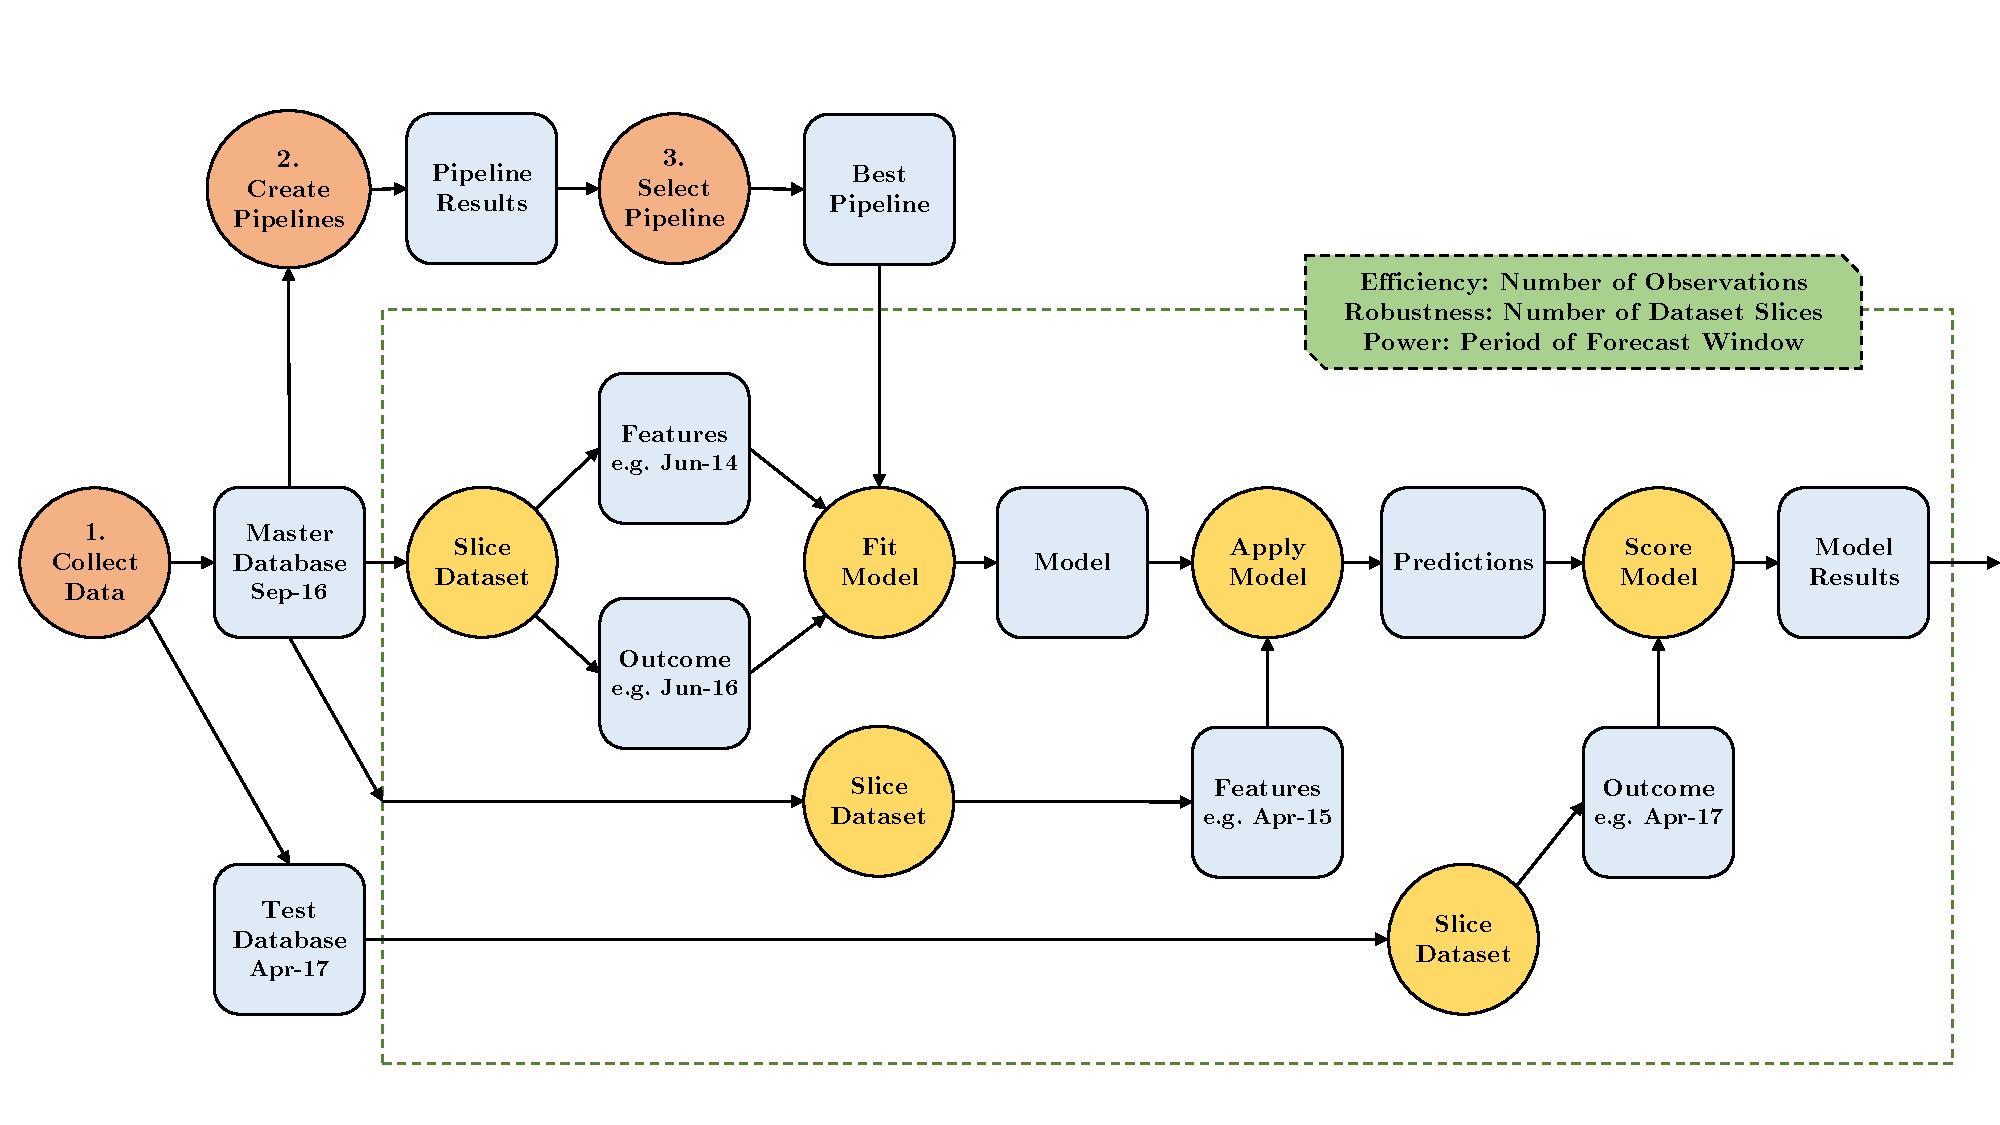
\includegraphics[width=\textwidth]{../figures/evaluation/pipeline_evaluation}
    \caption[Pipeline evaluation flowchart]{Pipeline evaluation overview.}
    \label{fig:evaluation:pipeline_evaluation}
\end{figure}

\subsection{Efficiency}

A rationale for this research project is the need for more efficient forms of \gls{vc} investment analysis which leverage technology, particularly in surfacing and screening. By its nature, our automated system should be more efficient than current manual methods but it's also important to determine how to most efficiently use the data that we have. For these reasons, we decided to investigate the learning curves for our classification pipeline to determine whether we could use smaller samples from our dataset to achieve similar predictive power and reduce our need for computational power and time taken. We used cross-validation to split our dataset 10 times and used subsets of the training set with varying sizes to train the estimator and produce training and test scores for each subset size. The convergence or divergence of our training and cross-validation curves will imply whether our classification pipeline is over- or under-fitting our data for various sizes allowing us to select an optimal sample size. We will also investigate the time profiling of the system to determine whether the system is practical for use in the \gls{vc} industry.


%TODO
%Figure Area under PR curves by training_observations
%Figure Time by training_observations

\subsection{Robustness}

It is critical that our system be robust with respect to time so investors can rely on its predictions based on historical models. CrunchBase provides created and last-updated timestamps for each record in their CSV-formatted dumps (and also in the JSON-formatted responses from their API). We took advantage of this to produce a system that reverse-engineers previous database states by filtering the current database by only records that were created by a given 'slice' date. We performed preliminary testing of this technique by comparing a historical CrunchBase database collected in December 2013 with a slice from our primary dataset collected in September 2016, as shown in Table~\ref{fig:evaluation:2013_slice_comparison}. While there are some differences in the records, particularly in the IPO relation, we consider this to be satisfactory variance considering the 3-year time period. The key relations for our purposes are Companies, Funding Rounds and People, all of which had minor differences considering the size of these datasets. Table~\ref{fig:evaluation:slice_counts_over_time} shows company counts by startup development stage from different dataset slices. We limited our experiments to dataset slices from 2012-onwards because prior to 2012 the datasets become too small to use to make predictions (particularly given the class imbalance).

\begin{figure}[!htb]
    \centering
    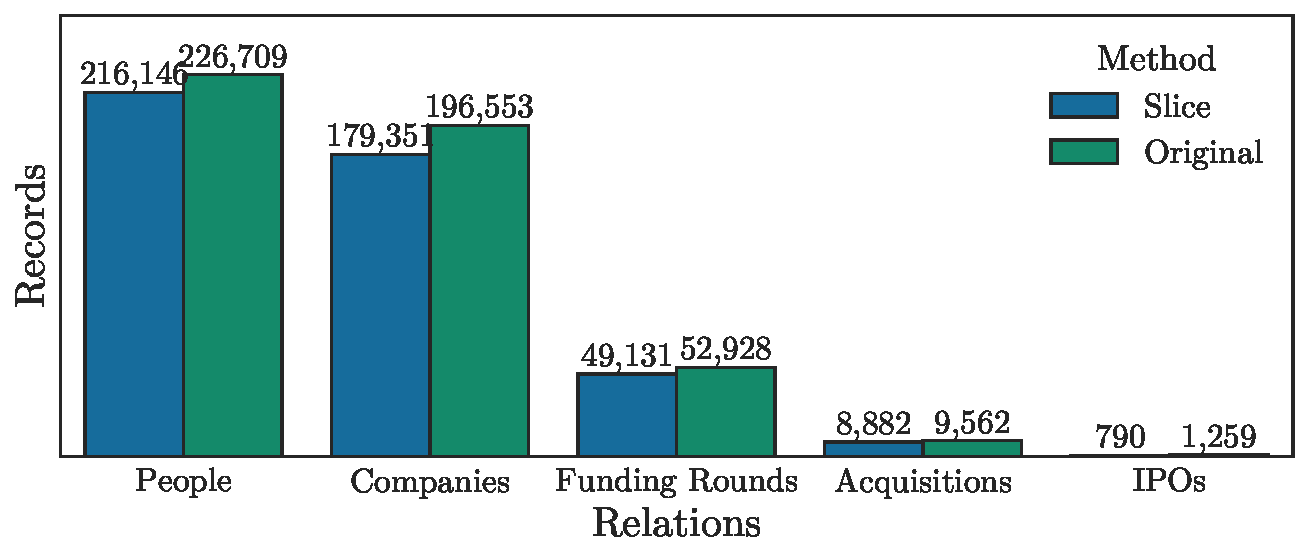
\includegraphics[width=\textwidth]{../figures/evaluation/2013_slice_comparison}
    \caption[Dataset slice compared with original dataset]{}
    \label{fig:evaluation:2013_slice_comparison}
\end{figure}

\begin{figure}[!htb]
    \centering
    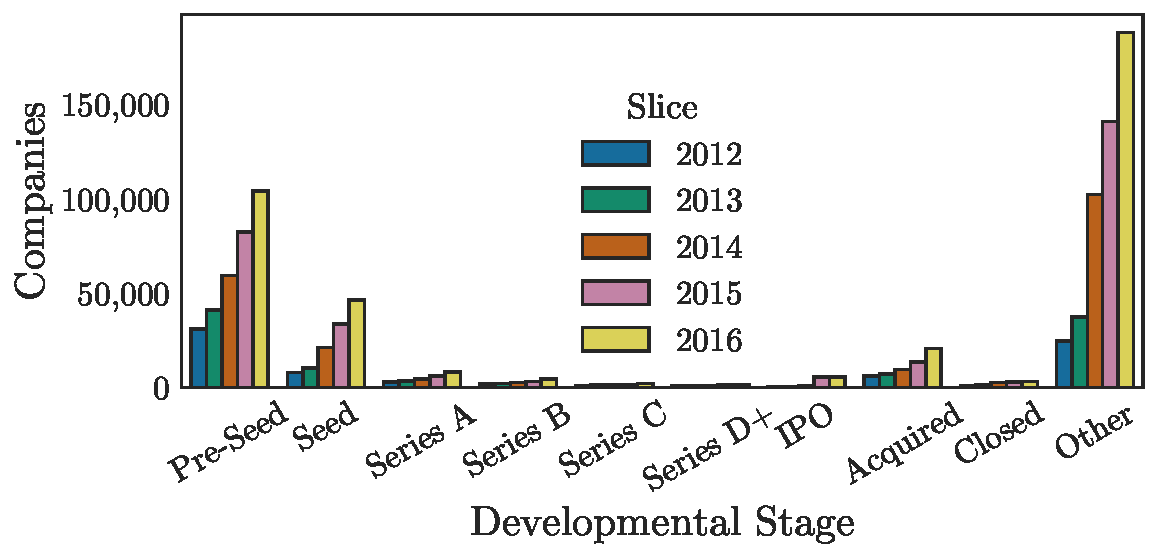
\includegraphics[width=\textwidth]{../figures/evaluation/slice_counts_over_time}
    \caption[Dataset counts over time]{}
    \label{fig:evaluation:slice_counts_over_time}
\end{figure}


%TODO
%Table Features ranked by importance by time slices.
%Figure PR curves for models trained by time slices (line plot).

\subsection{Predictive Power}

Finally, we test our system's predictive power for making forecasts of different time periods. We use the same system of reverse-engineering time slices that we used in our previous experiment to robustness, but this time we vary the time difference between the slice that provides our features and the slice that provides our label. We performed preliminary testing by combining pair-wise datasets of each year from 2012-2016 inclusive and exploring the proportion of companies that raised additional funding or exited (for brevity, we will call this ``investment success''.

Figure~\ref{fig:evaluation:outcome_forecast_window} shows how investment success varies with respect to the forecast window (time between the observed features and the measured outcome). Intuitively, we see a positive relationship between length of forecast window and investment success. In particular, very few companies appear to have investment success over a period of less than 2 years so we will focus our experimentation on forecast windows of 2--4 years.

\begin{figure}[!htb]
    \centering
    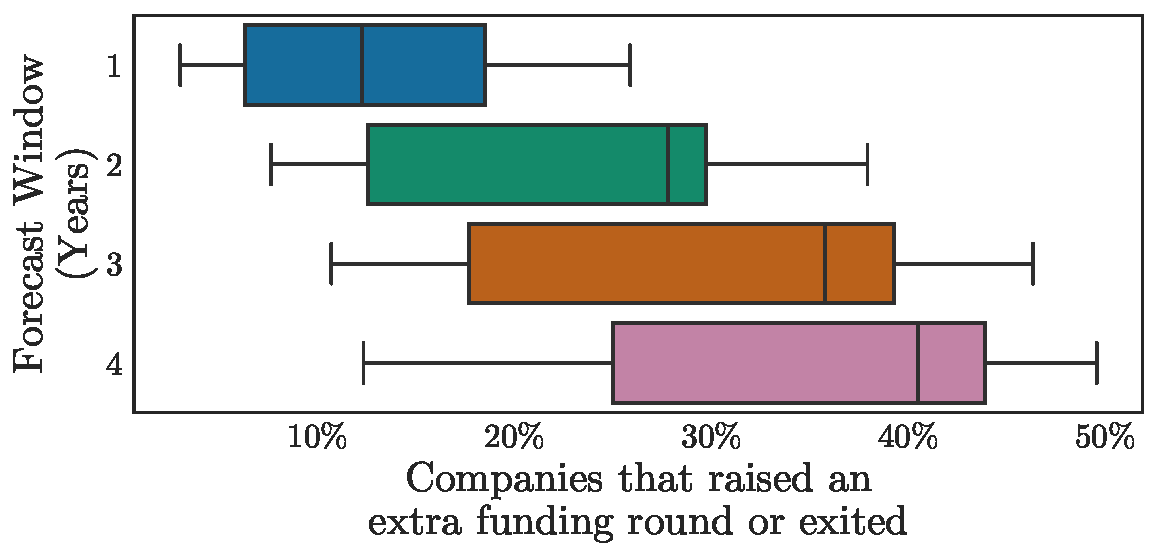
\includegraphics[width=\textwidth]{../figures/evaluation/outcome_forecast_window}
    \caption[Investment success by forecast window]{}
    \label{fig:evaluation:outcome_forecast_window}
\end{figure}

We also looked at how investment success varies with respect to development stage, shown in Figure~\ref{fig:evaluation:outcome_stage}. We see a broad positive relationship between developmental stage and likelihood of investment success, which we would expect as at each stage there is higher market traction and scrutiny from investors. One exception is for companies at Series D+ stage, but this may reflect that these companies are aiming for an exit which likely takes longer than seeking additional funding rounds and so is less well shown in our dataset (which caps out at a forecast window of 4 years). The variance between the different developmental stages suggests that in our experimentation we should investigate how our system predicts each stage independently, as well as in aggregate.

\begin{figure}[!htb]
    \centering
    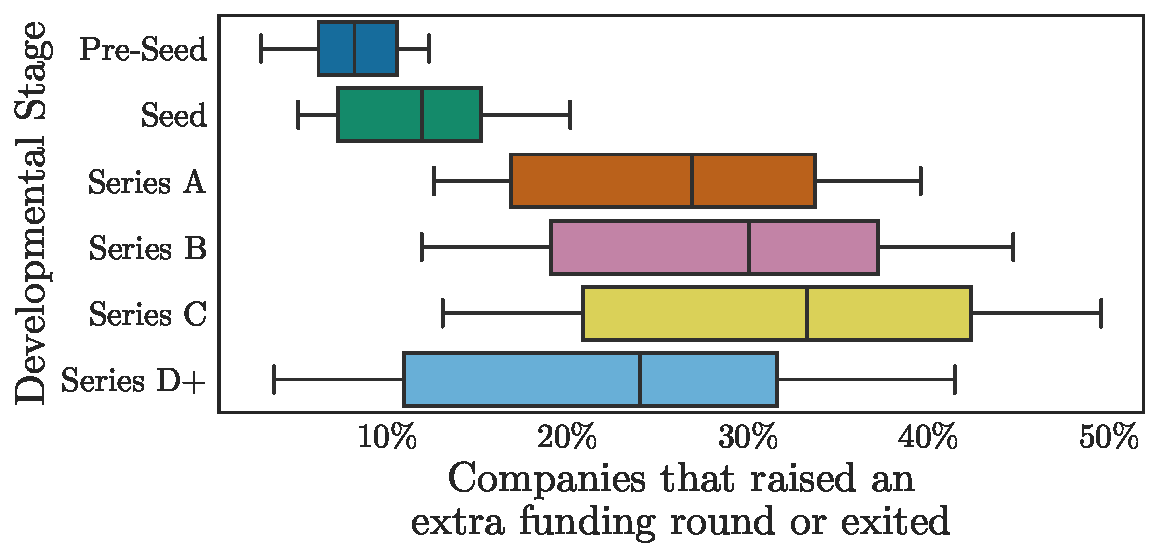
\includegraphics[width=\textwidth]{../figures/evaluation/outcome_stage}
    \caption[Investment success by developmental stage]{}
    \label{fig:evaluation:outcome_stage}
\end{figure}

%TODO
%Table Features ranked by importance by prediction windows.
%Figure PR curves for models by prediction windows (line plot).
%Figure PR curves for  companies by lifecycle stages (line plot).
%Figure Area under PR curves by lifecyle stage and prediction window (matrix)
%Table Three example company profiles and their predictions.

\section{Discussion}

%TODO

 \ifcsdef{mainfile}{}{\printbibliography}
\end{document}
